\documentclass[../ala_hataile.tex]{subfiles}
\begin{document}
\clearpage

\includepdf[pages=30-31, pagecommand={}]{sisasivut_19062018.pdf}
\twocolumn[\section{Geofysiikka}]
Geofysiikka on tiede, joka tutkii luonnon\-ilmiöitä fysiikan menetelmin Maan keski\-pisteestä aina lähi\-avaruuteen saakka. Yksi geo\-fysiikan parhaista puolista on sen konkreettinen läheisyys meitä ympäröivään luontoon. Geofyysikkona saat silloin tällöin heittää rinkan selkääsi ja suunnata jalkasi kenttä\-mittauksiin ja "-töihin. Luonnollisesti todellisen luonnon tutkiminen fysiikan keinoin vaatii myös runsaasti fysikaalista ja matemaattista perusosaamista, kova kenttä\-kunto ei pelkästään riitä. Geofysiikka on tärkeä ala myös ympäristötieteiden joukossa, sillä ympäristö\-ongelmien kokonaisvaltainen käsittely ei onnistu ilman geofysiikkaa.

Erityistä merkitystä geofysikaalinen osaaminen saa luonnonkatastrofien yhteydessä. Hyökyaallot ja tsunamit, tulivuorenpurkaukset, maanjäristykset, ilmastonmuutos ovat ongelmia jotka uhkaavat akuutisti laajoja väestönosia maapallolla. Ja vaikka meillä Suomessa näin suuren mittaluokan hasardeja ei olisikaan, niin silti tulvia, maaperän ja pohjavesien pilaantumista ja vastaavia alueellisia ongelmia esiintyy. Ihminen voi myös omalla toiminnallaan edes\-auttaa vaikkapa maanjäristysten syntyä -- myös täällä Suomessa -- ja kallioperän rakenteisiin ja fysikaalisiin ominaisuuksiin liittyy vielä paljon tieteelle avoimia kysymyksiä.

Tutkimuskohteidensa puolesta geofysiikka on kaksijakoinen tiede, eikä kaikilla meillä alan harjoittajilla ole suinkaan omaa lempikiveä. \textbf{Vesivaipan geofysiikka} kattaa hydrologian, fysikaalisen meritieteen ja glasiologian. \textbf{Kiinteän maan geofysiikan} alaisuuteen puolestaan kuuluvat geodesia, geomagnetismi, geotermiikka, seismologia ja sovellettu sekä planetaarinen geofysiikka. Opiskeltuasi pari geofysiikan kurssia kandivaiheessa on luontainen jatkosuunta Ilmakehätieteiden maisteriohjelma (ATM-MP) tai Geologian ja geofysiikan maisteriohjelma (Geo$^2$).

Jokaisen geofysiikasta kiinnostuneen
tulisi myös liittyä ainejärjestö Geysir~ry:n
jäseneksi saadakseen ajan tasalla olevan
vaikutus- ja tiedonkulkukanavan opintojen
tulevaisuudesta päättäviin tahoihin. Geysirin
hallituslaiset vastaavat mielellään kaikkiin
kysymyksiisi geofysiikan opiskelusta! Geysiriin kannattaa liittyä heti opiskelujen alussa, sillä jäsenyys on fukseille ilmainen. Käy myös liittymässä Facebook-ryhmäämme ja tykkäämässä yhteisösivustamme.

Ensimmäinen vuosi geofysiikan opiskelijoilla vierähtää tavallisesti fysiikan tai geotieteiden perusopintoja tehdessä. Matemaattisten ja laskennallisten menetelmien opiskelu on käytännössä välttämätöntä jo ensimmäisenä vuonna, sillä
niiden antamia tietoja (erit.\,vektorianalyysi, differentiaaliyhtälöt ja tieteellinen laskenta) tarvitaan jatkossa lähes jokaisella kurssilla. Varhaisin hetki, jolla geofysiikan kursseille kannattaa hypätä, on ensimmäisen vuoden nelosperiodissa, kun Matemaattiset apuneuvot on suoritettu ja Pythonista ja datankäsittelystä on jo vähän kokemusta.

Geofysiikan kanditasoiset kurssit on koottu aineopintopaketiksi FYS1800, johon kuuluvat mm.\,Meritieteen peruskurssi (``MerPe''), Hydrologian peruskurssi (``Hydro'') ja Kiinteän maan geofysiikan peruskurssi (``KMGP''). Geofysiikan opintokokonaisuus soveltuu matemaattisten ja teknillisten alojen, geotieteiden, luonnonmaantieteen ja ympäristötieteiden opiskelijoille, joilla on riittävät esitiedot. Helsingin yliopiston fysikaalisten tieteiden opiskelijat voivat sisällyttää geofysiikan kurssit Fysikaalisten tieteiden valinnaisten aineopintojen kurssipakettiin.

Muuten kurssit eivät edellytä
erityistä suoritusjärjestystä, eli liity vain
rohkeasti mukaan kokeilemaan, olisiko
geofysiikka sinun juttusi! Lisäksi geofysiikan
aineopinto- ja syvärikurssit voivat tuoda vaihtelua ja virkistystä
myös muille kuin varsinaisille geofyssan opiskelijoille.

Lisätietoja vesivaipan geofysiikan opinnoista
voit kysyä esimerkiksi prof.\,Petteri Uotilalta (Exactum~B112) ja yli\-opisto\-lehtori Ivan Mammarellalta (Exactum~D116). Kiinteän maan opiskelusta lisätietoa
antavat prof.\,Ilmo Kukkonen (Exactum~D432), apulaisprofessori David Whipp (Exactum~D430) sekä yli\-opisto\-lehtori Emilia Koivisto (Exactum~D431).

Terveisin geofysiikan tuutorit ja fuksi- ja
tuutorivastaavat

\vspace{0.5cm}
\noindent\textsc{Bláthnaid}\\
\textsc{Sakke}\\
\textsc{Tomas}
\vspace{1cm}

\subsection*{Geofysiikan kursseja kanditutkintoon}
\subsubsection*{Meritieteen peruskurssi (5~op)}
Meritieteen peruskurssi, tuttavallisemmin
MerPe, antaa yleiskuvan fysikaalisesta
meritieteestä. Aiheet vaihtelevat meriveden
ominaisuuksista suolaisuus- ja lämpöoloihin,
virtauksiin, aaltoihin, meren ja ilman
vuorovaikutukseen ja merijäähän. Laskuharjoitukset
ovat kerran viikossa.

Alan esitietoja ei vaadita, vaan lukion
pitkällä fysiikalla ja matematiikalla pääsee
pitkälle. Matemaattiset apuneuvot~I--III
totuttavat kuitenkin kurssilla vaadittavaan
laskurutiiniin. Tämän vuoksi kurssi sopii
hyvin myös fysikaalisesti orientoituneille geotieteilijöille,
maantieteilijöille, matemaatikoille, kemisteille
sekä biologeille. Kurssi on osa geofysiikan opintokokonaisuuden
pakollisia aineopintoja ja suositeltava myös meteorologeille.

\subsubsection*{Hydrologian peruskurssi (5~op)}
Kurssilla käsitellään veden kiertokulkua
luonnossa. Järvien ja jokien fysikaaliset
ominaisuudet ja prosessit, sekä maaperän
vedet tulevat tutuiksi kurssin aikana. Laskuharjoitukset
ovat kerran viikossa.

Hydro on kohtuullisen vähätöinen kurssi
eikä vaadi juuri lainkaan matemaattista
tuskailua. Kurssin aiheet sivuavat vahvasti Meteorologian
ja säähavainnonteon perusteita. Nämä
kaksi ovatkin mukava kombo fuksivuoden
keväällä suoritettavaksi innokkaille geofyysikon
aluille. Meritieteen tavoin myös
Hydrologian peruskurssi soveltuu mainiosti
muidenkin koulutusohjelmien luonnontieteilijöille
oman kiinnostuksen mukaan.

\subsubsection*{Kiinteän maan geofysiikan peruskurssi (5~op)}
Kurssi tarjoaa kattavan kuvan kiinteän
maan geofysiikasta ja avaa yhdessä geotieteiden ja fysiikan
perusopintojen kanssa portin Geologian ja geofysiikan maisteriohjelmaan (Geo$^2$). Kurssin kohderyhmänä
ovat 2.\,tai 3.\,vuoden
geotieteilijät ja fyysikot.
Osa-alueina ovat mm.\,laatta\-tektoniikka,
geodesia, seismologia, geo\-magnetismi,
maan lämpö\-olo\-suhteet sekä radio\-aktiivinen
ajan\-määritys.
\begin{figure}[b!]
	\centering
	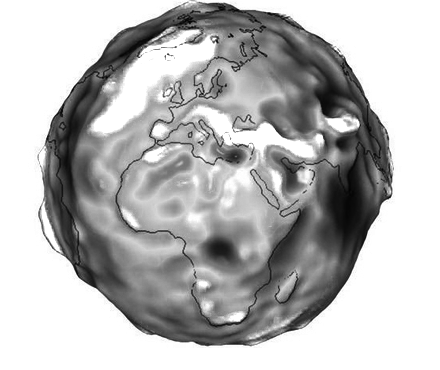
\includegraphics[width=\columnwidth]{Earth_gravity.png}
\end{figure}

KMGP luennoidaan Powerpoint-sulkeisilla
lasku\-harjoituksineen. Kurssin keskeisintä antia ovat perustavan\-laatuiset tiedot Maapallon sisä\-rakenteesta ja toiminnasta sekä opastus terveeseen
akateemiseen kriittisyyteen ja varovaiseen tiedon\-arviointiin. Kurssikirja (Fowlerin
``The Solid Earth: an Introduction to Global
Geophysics'') on tiukkaa tekstiä ja hyvä
viite\-teos koko myöhemmälle elämälle, ja
sen hankkimista kirja\-hyllyn koristeeksi
voidaan lämpimästi suositella.

\subsubsection*{Virtausilmiöt (5~op)}
Kurssilla katsellaan kuvia hassuista virtausrakenteista kuten virtauksesta sylinterin ohi, alhaisen ja korkean Reynoldsin luvun virtauksesta sekä vapaasta konvektiosta. Kurssilla opitaan myös, mitä ovat virtafunktiot, trajektorit, pyörteisyys ja sirkulaatio. Aiheet ovat ilmeisen päällekkäiset ilmakehän dynamiikan kurssien kanssa, mutta tällä kurssilla matemaattiseen puoleen ei sukelleta yhtä syvälle.

\subsection*{Maisteriohjelmien maistelukursseja}
\subsubsection*{Oceanography of the Baltic Sea (5~op)}
Kursseilla käsitellään Itämeren oseanografian
pääpiirteet eli hydrografia, kiertoliike,
lämpötalous ja jääpeite. Lisäksi
käsitellään mittausmenetelmiä ja mallinnusta,
sekä tutustutaan fysikaalisten ja ekologisten
tekijöiden yhteyksiin. Kurssikirja
``Itämeren fysiikka, tila ja tulevaisuus'' on
hyvä käsikirja ja kattaa täysin
kurssin aihealueet. Pohjalle suositellaan Meritieteen peruskurssia.

\subsubsection*{Geophysics of Snow and Ice (5~op)}
Kurssi alkaa jään kiderakenteeseen tutustumisesta, minkä jälkeen käsitellään lunta kaikissa olomuodoissa ja kaikissa ympäristöissä, missä sitä Maapallolla esiintyy. Kurssin lopussa on kahden päivän mittainen kenttäosuus Lammilla, jossa opitaan kaivamaan lumikuoppa ja sahaamaan näytteitä järvijäästä ja tarkastelemaan niitä polarisaatiolevyjen välissä.

\subsubsection*{Solid State Continuum Mechanics~I (5~op)}
Jatkumomekaniikka on oppi kiinteän aineen käyttäytymisestä jännityksen ja venymän alla. Kurssilla on neljä luennoijaa, jotka kukin tarkastelevat aihetta hieman eri näkökulmasta: teoreettisesta, kokeellisesta, laskennallisesta ja taloudellisesta. 

Teoreettisessa osuudessa pyöritellään tensoreita aina neljänteen kerta\-lukuun asti, ja laskennallisessa osuudessa hakataan päätä seinään Fortranilla kirjoitettujen black boxien kanssa. Kotiharjoitukset ovat pieniä analyyttisiä tai laskennallisia ongelmia, ja loppu\-harjoituksessa tutkitaan ääni\-raudan värähtelyä neljällä eri tavalla ja kirjoitetaan siitä tutkimus\-raportti. 

Tämän kurssin jälkeen Seismologian opintojen pitäisi olla kuin lasten leikkiä.

\subsection*{Minustako geofyysikko?}
Lisätietoa kursseista ja muista tärkeistä
geofysiikkaan liittyvistä asioista löydät
WebOodista sekä Ilmakehätieteiden maisteriohjelman ja Geo$^2$-maisteri\-ohjelman kotisivuilta.

Kiinteän maan maisteriohjelman sähköpostilista
on \url{seg-people@helsinki.fi}, johon
pääsee lähettämällä Majordomoon viestin
``subscribe seg-people'' ilman lainausmerkkejä
ja otsikkokenttää. Lisäksi voit kääntyä
geofysiikan opiskelijoiden puoleen esimerkiksi
Geysirin kautta, lisätietoa \url{http://blogs.helsinki.fi/geysir-ry}.

\vspace{0.5cm}
\noindent
\textsc{Sakari Väkevä}\\
\textsc{Joula Siponen}\\
\textsc{Veera Leppänen}\\
\textsc{Hedi Kanarik}\\
\textsc{Kaiu Piipponen}
\end{document}